\documentclass[10pt,conference,compsocconf]{IEEEtran}

\usepackage{hyperref}
\usepackage{graphicx}	% For figure environment
\usepackage{amsmath}
\usepackage{placeins}

\begin{document}
\title{ML Project 2 - Report}

\author{
  Sarah Mikami, Samuel Waridel and Florian Kolly \\
  \textit{CS433, EPFL 2024}
  \textit{ML4Science project | TNE Laboratory}
}

\maketitle

\begin{abstract}

\end{abstract}

\section{Introduction}
Machine Learning (ML) is has become a central tool in neuroscience, with applications in neural engineering (e.g. Brain-Computer Interfaces, BCIs), diagnostics and fundamental research. For instance, Jalilifard et al. \cite{EmotionClassificationSVM} demonstrated the efficacy of Support Vector Machine (SVM) classifiers in basic emotions recognition, while Bose et al. \cite{EEGRandomForset} used Random Forest classifiers to automate seizure detection in epileptic patients with high accuracy. Indeed, all major ML methods have been applied to neural signals classification\cite{EEGMLReview}.

In this work, we examine the applications of such ML techniques in three classification problems using sEEG signals: i) distinguishing between the execution and observation of a movement; ii) differentiating between grasping a small versus a large object; iii) differentiating between observing the grasp of a small versus a large object.

Section \ref{sec:problem} outlines the data acquisition process and its relevance to our classification tasks. In Section \ref{sec:analysis}, we describe the preprocessing of the sEEG signals and the extraction of relevant features. Sections \ref{sec:actionrecognition} and \ref{sec:objectrecognition} present the models applied to our classification problems and their performance. In Section \ref{sec:deeplearning}, we explore the idea of using only Deep Learning (DL) to directly extract features from the EEG signal. Finally, we discuss our results in Section \ref{sec:discussion} and conclude in Section \ref{sec:conclusion}.

\section{Data acquisition and problem specification}
\label{sec:problem}
The dataset comprises signals recorded from four participants, each implanted with sEEG electrodes in distinct brain regions. During multiple experimental sessions, participants were instructed to either observe or execute specific motor tasks. These tasks involved two types of movements: a palmar grasp (force-based movement) and a pinch grasp (precision-based movement). Each session included multiple trials structured as follows: in an execution trial, the trial begins with a start cue. One second later, a light cue signals the type of object (small or large) to be targeted. This light remains illuminated for 0.5 seconds before turning off. After an additional 1.5 seconds, a "go" signal prompts the participant to lift their hand from the resting position, grasp the indicated object, return it to its original location, and place their hand back in the resting position. Observation trials followed an identical structure, except that participants passively observed the experimenter performing the actions. A light cue indicated the participant's role (execution or observation) in each trial.

\begin{figure}[h!]
  \center
  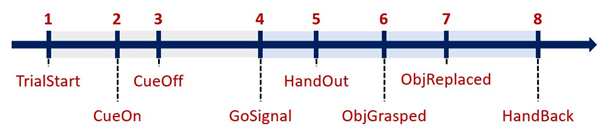
\includegraphics[width=\linewidth]{images/2024-12-11-13-41-48.png}
  \caption{Timing of the trials}
\end{figure}
\FloatBarrier

\section{Data analysis}
\label{sec:analysis}

\subsection{Channel responsiveness}
Which regions have the most responsive channels, are they the same for execution \& obervation?

\begin{itemize}
    \item Across participant: same region? same nb of responsive channels?
    \item Are the channels responsive for obs also responsive for ex? Vice-versa?
    \item Do we find the expected regions? Link to mvt execution / observation?
\end{itemize}

For channels where we have response for both ex \& obs, are the responses congruent (similar pattern) or incongruent (different)?

\begin{itemize}
    \item Amplitude, shape of response \(\to\) difference?
    \item Response pattern at the same timing?
    \item Similar frequency characteristics?
    \item Correlation? High correlation suggests congruence
    \item Are the results obtained similar for both movements?
\end{itemize}


\section{Action recognition}
\label{sec:actionrecognition}
Do it for each participants

\subsection{Models}
\paragraph{SVM}
\paragraph{Random forest}
\paragraph{MLP}
\subsection{Results}
\subsection{Discussion}
Which freq. bands are important? Is it the same across subjects?

\section{Object recognition}
\label{sec:objectrecognition}
Do it for each participants

\subsection{Models}
\paragraph{SVM}
\paragraph{Random forest}
\paragraph{MLP}

\subsection{Results}
\subsection{Discussion}
Which freq. bands are important? Is it the same across subjects?

\section{Pure deep learning approach}
\label{sec:deeplearning}
Can a 1D conv. network learn relevant features for classification? Create and test model on trials themselves

\section{Discussion}
\label{sec:discussion}

\section{Conclusion}
\label{sec:conclusion}


%%%%%%%%%% ETHICAL RISKS %%%%%%%%%%
%% 200 to 400 words max., does not count in the 4-page limit
\section{Ethical risks}




%% Not in the 4-page limit
\section{Appendix}

\begin{figure}[h!]
    \center
    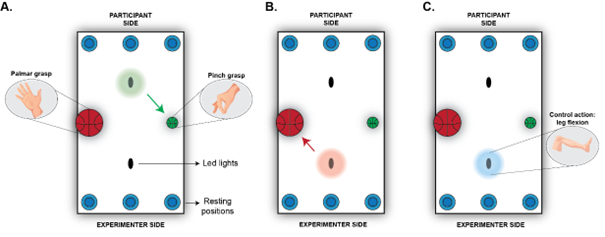
\includegraphics[width=\linewidth]{images/2024-12-11-13-41-23.png}
    \caption{Experimental setup}
\end{figure}
\FloatBarrier


% \begin{figure}[tbp]
%   \centering
%   \includegraphics[width=\columnwidth]{denoised_signal_1d}
%   \caption{Signal compression and denoising using the Fourier basis.}
%   \vspace{-3mm}
%   \label{fig:denoise-fourier}
% \end{figure}


\section*{Acknowledgements}
We thank Leonardo Pollina for taking us with him on this project, and for his quick and helpful answers to all our questions.

\bibliographystyle{IEEEtran}
\bibliography{ref}

\end{document}

% <a href="https://www.vecteezy.com/free-vector/brain-diagram">Brain Diagram Vectors by Vecteezy</a>